\section{Analysing Traffic Characteristics}\label{sec:traffic}

As reported in previous research~\cite{Sarrar:2012}, network traffic follows a Zipf distribution.
Indeed, several research has demonstrated that network flows monopolizes the a huge slice of the whole traffic.

In our study, we have re-conducted experiments to determine the traffic characteristics of a up-to-date real-world data center trace.
We have replayed a CAIDA network trace extracted from an IXP in a data center in New York~\cite{caida:19}.
Astute readers will notice that similar analysis has been done by~\citeauthor{Spang:19} to estimate number of TCP/IP flows~\cite{Spang:19}.
The analysed trace is 1 minute long monitoring a full-duplex \SI{40}{\giga\bit/\second} link connecting New York and S\~ao Paulo/Brazil.
Figure~\ref{fig:traces} summarizes our observations. In our analysis, a flow is characterized by a unique five tuple $\langle$~IPv4/IPv6 Source IP address, IPv4/IPv6 destination IP address, L4 protocol, UDP/TCP source port, UDP/TCP destination port~$\rangle$ connection.

\begin{figure*}[]
\centering
\subfloat[Heavy hitter analysis]{
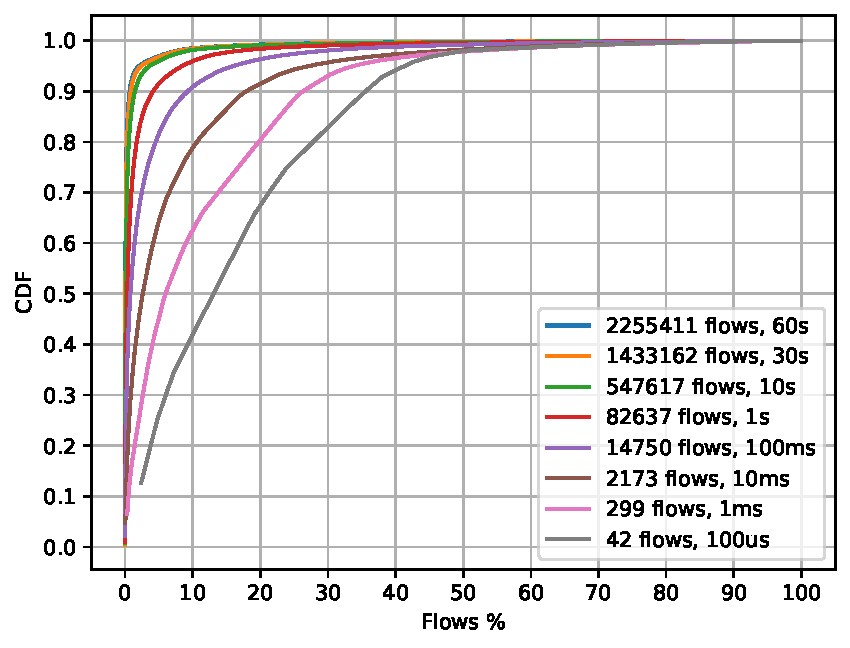
\includegraphics[width=0.33\textwidth]{fig_cdf.pdf}
\label{fig:cdf}
}
\subfloat[Flow duration]{
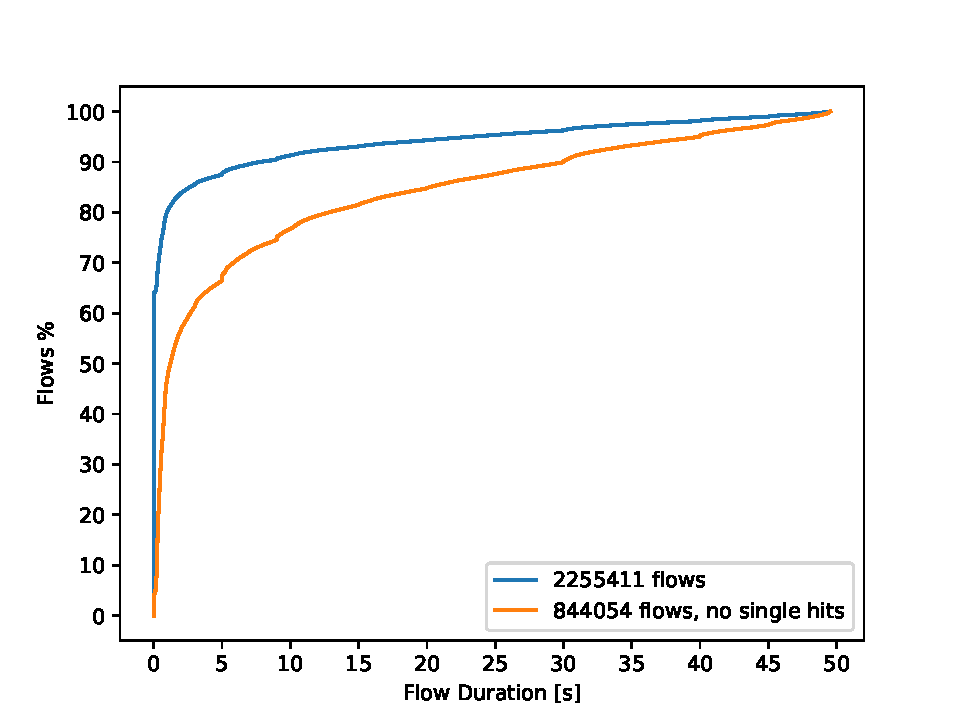
\includegraphics[width=0.33\textwidth]{fig_duration.pdf}
\label{fig:flow_duration}
}
\subfloat[Average flow size]{
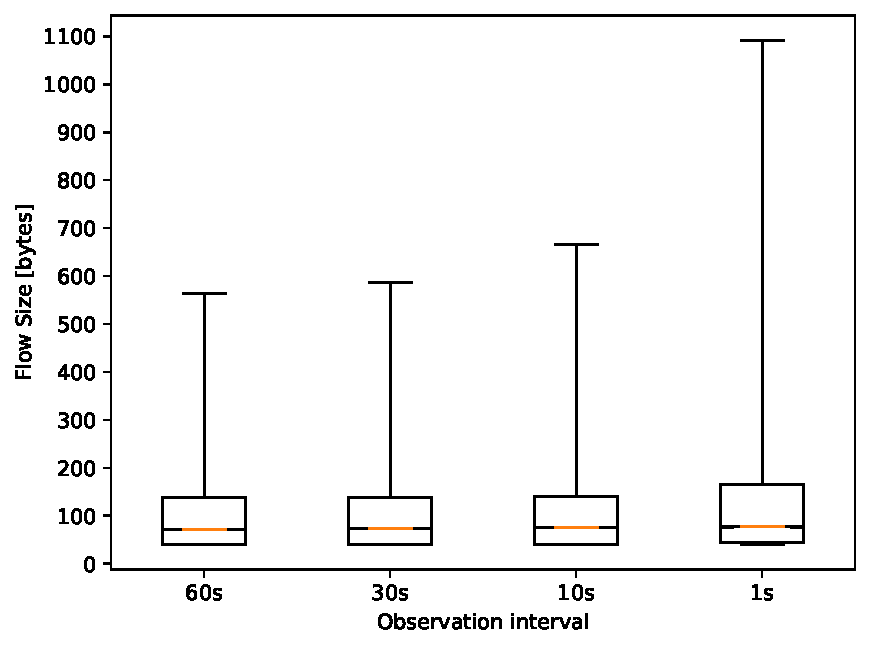
\includegraphics[width=0.33\textwidth]{fig_avg_flow_size.pdf}
\label{fig:flow_size}
}
\caption{CAIDA trace summary}
\label{fig:traces}
\end{figure*}

As we observe in Figure~\ref{fig:cdf}, Zipf's characteristic is still present in current network traffic.
In the figure, we present the CDF, in terms of transmitted bytes, for several observation intervals, ranging from \SI{100}{\micro\second} to \SI{60}{\second}.
For all observation intervals longer than \SI{100}{\milli\second}, more than 10\% of the flows dominate more than 90\% of the traffic.
For shorter intervals, the dominance is presented however less evident.

In Figure~\ref{fig:flow_duration}, we present the flow duration time.
The blue curve is dominated (60\%) by single packet flows.
These single packet flows are represented in the graph with a flow duration of zero.
Still in the blue curve, we observe the short-lived flows dominate the trace with $\sim$90\% of all flows during less than 5 seconds.
The orange curve in Figure~\ref{fig:flow_duration} illustrates the flow duration of flows with multiple hits in the trace.
Still, short-lived flows dominate the trace with $\sim$50\% lasting less than 1 second in the trace.

Figure~\ref{fig:flow_size} presents the average flow size for four statistically representative observation intervals.
For all four measures, the first quartile, the median, and the third quartile are very similar.
On average, short flows ($\sim$100 bytes) dominates the trace with 75\% of the flows are no bigger than 150 bytes.

According to our experiments, the zipf pattern is still present on current data center traffic.
Such characteristic favors flow caching in memory scarce programmable dataplanes.
However, we notice that short-lived flows dominate the trace and therefore the caching policy algorithm needs fast reaction time in order to adapt to traffic changes.
In addition, such temporal traffic characteristic will probably favor time-based cache policies (e.g. LRU).

\section{Cache Replacement Algorithms}\label{sec:policies}

\paragraph{LRU}
The LRU replacement algorithm evicts the most ancient cache entry in case of a cache miss.
A possible LRU implementation would use a timestamp tag to sort cache entries by recency, as in Algorithm~\ref{algo:lru}.

\begin{algorithm}[]
	\caption{LRU policy}
	\label{algo:lru}
	\SetInd{0.1em}{.9em}
	\SetAlgoLined
	\footnotesize
	\SetKwProg{procedure}{Procedure}{}{end}
	\SetKwFunction{minTimestampEntry}{minTimestampEntry}
	\SetKwFunction{findEntry}{findEntry}
	\SetKwFunction{lruPolicy}{lruPolicy}
	\SetKwInOut{Input}{input}
	\SetKw{In}{in}%
	\SetKw{Not}{not}%
	\SetKw{Or}{or}%
	\SetKw{Continue}{continue}%
	\SetKw{True}{true}%
	\Input{Cache memory: list of $\langle$\texttt{entry, timestamp}$\rangle$ pairs}
	\Input{Possible cache entry}
	\Input{Packet timestamp}
	\procedure{\lruPolicy{cache, possible\_entry, current\_timestamp}}{
		
		\tcc{Check for a cache hit}
		\If{possible\_entry \In cache}{
			\tcc{Get a pointer to the hit entry}
			entry\_found =  \findEntry{cache, possible\_entry}
			
			\tcc{Updates the timestamp}
			entry\_found$\rightarrow$timestamp  = current\_timestamp
		}
		\tcc{Cache miss}
		\Else{
			\tcc{Get a pointer to the victim}
			victim =  \minTimestampEntry{cache}
			
			\tcc{Updates the entry}
			*victim = $\langle$possible\_entry, current\_timestamp$\rangle$
		}
	}
\end{algorithm}

\paragraph{LFU}

Contrary to LRU, LFU uses hit frequency rather than the access time to evict entries.
LFU uses a frequency counter to sort cache entries by frequency.
In case of a hit, the frequency counter is incremented.
Otherwise, the cache entry with the lowest frequency is chosen as victim, as in Algorithm~\ref{algo:lfu}.

\begin{algorithm}[]
	\caption{LFU policy}
	\label{algo:lfu}
	\SetInd{0.1em}{.9em}
	\SetAlgoLined
	\footnotesize
	\SetKwProg{procedure}{Procedure}{}{end}
	\SetKwFunction{lfuPolicy}{lfuPolicy}
	\SetKwFunction{findEntry}{findEntry}
	\SetKwFunction{minFrequencyEntry}{minFrequencyEntry}
	\SetKwInOut{Input}{input}
	\SetKw{In}{in}%
	\SetKw{Not}{not}%
	\SetKw{Or}{or}%
	\SetKw{Continue}{continue}%
	\SetKw{True}{true}%
	\Input{Cache memory: list of $\langle$\texttt{entry, counter}$\rangle$ pairs}
	\Input{Possible cache entry}
	\procedure{\lfuPolicy{cache, possible\_entry}}{
		
		\tcc{Check for a cache hit}
		\If{possible\_entry \In cache}{
			\tcc{Get a pointer to the hit entry}
			entry\_found =  \findEntry{cache, possible\_entry}
			
			\tcc{Updates frequency counter}
			entry\_found$\rightarrow$counter  += 1
		}
		\tcc{Cache miss}
		\Else{
			\tcc{Get a pointer to the victim}
			victim =  \minFrequencyEntry{cache}
			
			\tcc{Updates the entry}
			*victim = $\langle$possible\_entry, 1$\rangle$
		}
	}
\end{algorithm}

\paragraph{Random}

Random or pseudo-random replacement policies use an stochastic random function to select a victim for cache replacement.
Pseudo-random has been widely adopted in ARM-based processors.
In random policies, no history on cache misses/hits is required.
The efficiency of a random policy is directly related to the quality of its random generator function.

\paragraph{OPT}

\paragraph{WLFU}
As observed in previous research~\cite{Kim:09}, \textit{vanilla} implementations of LFU perform poorly with real-world network traces.
Original LFU considers all cache hits with equal weight, which is not true in network communications, where larger packets incur in greater network efficiency compared to small ones.
Thus, Weighted LFU (WLFU) differs from \textit{vanilla} LFU by considering the packet size in its frequency counters, as shown in Algorithm~\ref{algo:wlfu}.

\begin{algorithm}[]
\caption{WLFU policy}
\label{algo:wlfu}
\SetInd{0.1em}{.9em}
\SetAlgoLined
\footnotesize
\SetKwProg{procedure}{Procedure}{}{end}
\SetKwFunction{wlfuPolicy}{wlfuPolicy}
\SetKwFunction{findEntry}{findEntry}
\SetKwFunction{minFrequencyEntry}{minFrequencyEntry}
\SetKwInOut{Input}{input}
\SetKw{In}{in}%
\SetKw{Not}{not}%
\SetKw{Or}{or}%
\SetKw{Continue}{continue}%
\SetKw{True}{true}%
\Input{Cache memory: list of $\langle$\texttt{entry, counter}$\rangle$ pairs}
\Input{Possible cache entry}
\Input{Packet Size}
\procedure{\wlfuPolicy{cache, possible\_entry, pkt\_size}}{

	\tcc{Check for a cache hit}
	\If{possible\_entry \In cache}{
		\tcc{Get a pointer to the hit entry}
		entry\_found =  \findEntry{cache, possible\_entry}

		\tcc{Updates frequency counter with the packet size}
		entry\_found$\rightarrow$counter  += pkt\_size
	}
	\tcc{Cache miss}
	\Else{
		\tcc{Get a pointer to the victim}
		victim =  \minFrequencyEntry{cache}
	
		\tcc{Updates the entry}
		*victim = $\langle$possible\_entry, pkt\_size$\rangle$
	}
}
\end{algorithm}

\paragraph{OLFU}
Again, Optmistic LFU (OLFU) is a proposition to overcome the limitations of \textit{vanilla} LFU for flow caching.
OLFU is a an LFU derivation that gives a chance for a cache promotion candidate to remain in cache regardless its \textit{actual} hit frequency.
In case of a cache hit, OLFU behaves as the original LFU.
Otherwise, instead of re-initializing the frequency counter, the new cache entry takes control of the victim counter, as show in Algorithm~\ref{algo:olfu}.

\begin{algorithm}[]
\caption{OLFU policy}
\label{algo:olfu}
\SetInd{0.1em}{.9em}
\SetAlgoLined
\footnotesize
\SetKwProg{procedure}{Procedure}{}{end}
\SetKwFunction{olfuPolicy}{olfuPolicy}
\SetKwFunction{findEntry}{findEntry}
\SetKwFunction{minFrequencyEntry}{minFrequencyEntry}
\SetKwInOut{Input}{input}
\SetKw{In}{in}%
\SetKw{Not}{not}%
\SetKw{Or}{or}%
\SetKw{Continue}{continue}%
\SetKw{True}{true}%
\Input{Cache memory: list of $\langle$\texttt{entry, counter}$\rangle$ pairs}
\Input{Possible cache entry}
\procedure{\olfuPolicy{cache, possible\_entry}}{

	\tcc{Check for a cache hit}
	\If{possible\_entry \In cache}{
		\tcc{Standard LFU frequency update procedure}
	}
	\tcc{Cache miss}
	\Else{
		\tcc{Get a pointer to the victim}
		victim =  \minFrequencyEntry{cache}
	
		\tcc{Updates the entry}
		*victim = $\langle$possible\_entry, victim$\rightarrow$counter + 1$\rangle$
	}
}
\end{algorithm}


\paragraph{OWLFU}
OWLFU is a combination of OLFU and WLFU aiming at increasing the efficiency of LFU-based policies.
In case of a hit, OWLFU behaves as WLFU.
Otherwise, OWLFU modifies OLFU by incrementing the current packet size to the victim frequency counter, as in Algorithm~\ref{algo:owlfu}.

\begin{algorithm}[]
\caption{OWLFU policy}
\label{algo:owlfu}
\SetInd{0.1em}{.9em}
\SetAlgoLined
\footnotesize
\SetKwProg{procedure}{Procedure}{}{end}
\SetKwFunction{owlfuPolicy}{owlfuPolicy}
\SetKwFunction{findEntry}{findEntry}
\SetKwFunction{minFrequencyEntry}{minFrequencyEntry}
\SetKwInOut{Input}{input}
\SetKw{In}{in}%
\SetKw{Not}{not}%
\SetKw{Or}{or}%
\SetKw{Continue}{continue}%
\SetKw{True}{true}%
\Input{Cache memory: list of $\langle$\texttt{entry, counter}$\rangle$ pairs}
\Input{Possible cache entry}
\Input{Packet Size}
\procedure{\owlfuPolicy{cache, possible\_entry, pkt\_size}}{

	\tcc{Check for a cache hit}
	\If{possible\_entry \In cache}{
		\tcc{WLFU frequency update procedure}
	}
	\tcc{Cache miss}
	\Else{
		\tcc{Get a pointer to the victim}
		victim =  \minFrequencyEntry{cache}
	
		\tcc{Updates the entry}
		*victim = $\langle$possible\_entry, victim$\rightarrow$counter + pkt\_size$\rangle$
	}
}
\end{algorithm}

\section{Evaluating Cache Policies}\label{sec:cache_results}

\subsection{Experimental Setup}
We present the cache performance for different policies and cache sizes, as presented in Table~\ref{tab:setup}.
In addition, we have simulated the cache performance by emulating different cache policer reaction times.
As performance metrics, we report the cache hit ratio and the traffic size weighted hit ratio.
We use the term slowdown factor to refer to the policer reaction time.
The slowdown factor is relative to the cache speed, i.e., a slowdown of 10 means that the cache policer is 10 times slower than a cache access.
To enable reproducibility, we open-source our codes\footnote{\url{https://github.com/engjefersonsantiago/Infinite_MT}.}.

\begin{table}[]
	\centering
	\caption{Experimental Parameters}
	\label{tab:setup}
	\begin{tabular}{|l|l|}
		\hline
		\textbf{Parameter}       & \textbf{Value}   \\
		\hline
		Cache policy            & LRU, (O)(W)LFU, Random			    \\
		Cache Size              & 64 to \SI{8}{\kilo\nothing} entries  \\
		Slowdown Factor         & 1, 10, 100        \\
		\hline
	\end{tabular}
\end{table}

\subsection{Results}
Figure~\ref{fig:hit_ratio} presents the results for our experiments.

\begin{figure*}[]
\centering
\subfloat[Hit Ratio. Slowdown factor = 1]{
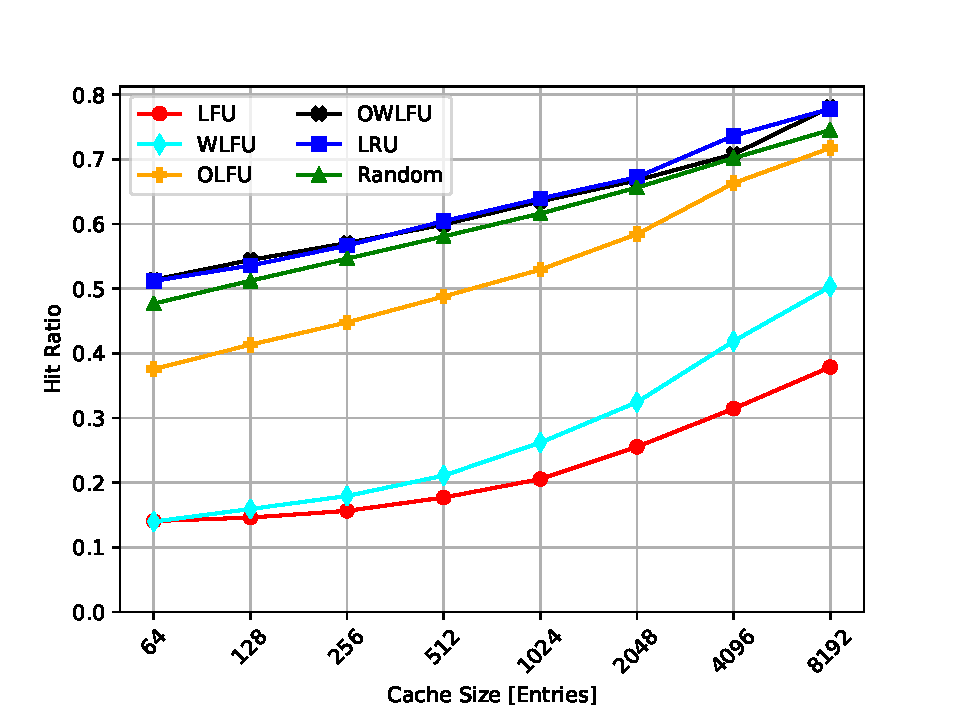
\includegraphics[width=0.33\textwidth]{hit_ratio_sf1.pdf}
\label{fig:hit_ratio_sf1}
}
\subfloat[Hit Ratio. Slowdown factor = 10]{
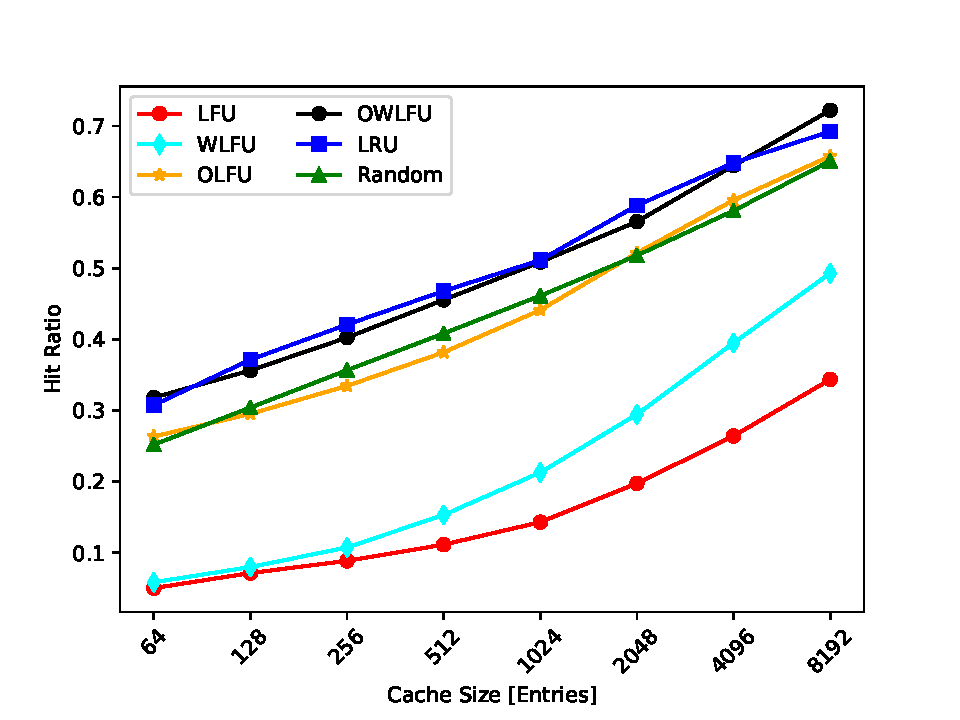
\includegraphics[width=0.33\textwidth]{hit_ratio_sf10.pdf}
\label{fig:hit_ratio_sf10}
}
\subfloat[Hit Ratio. Slowdown factor = 100]{
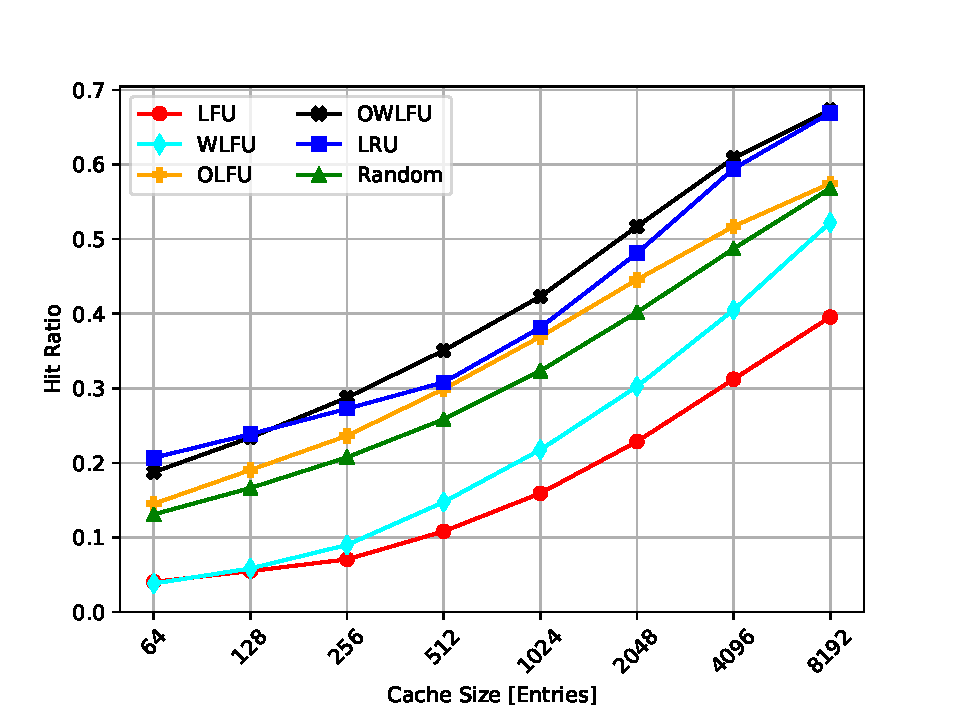
\includegraphics[width=0.33\textwidth]{hit_ratio_sf100.pdf}
\label{fig:hit_ratio_sf100}
}\\
\subfloat[Size Weighted Hit Ratio. Slowdown factor = 1]{
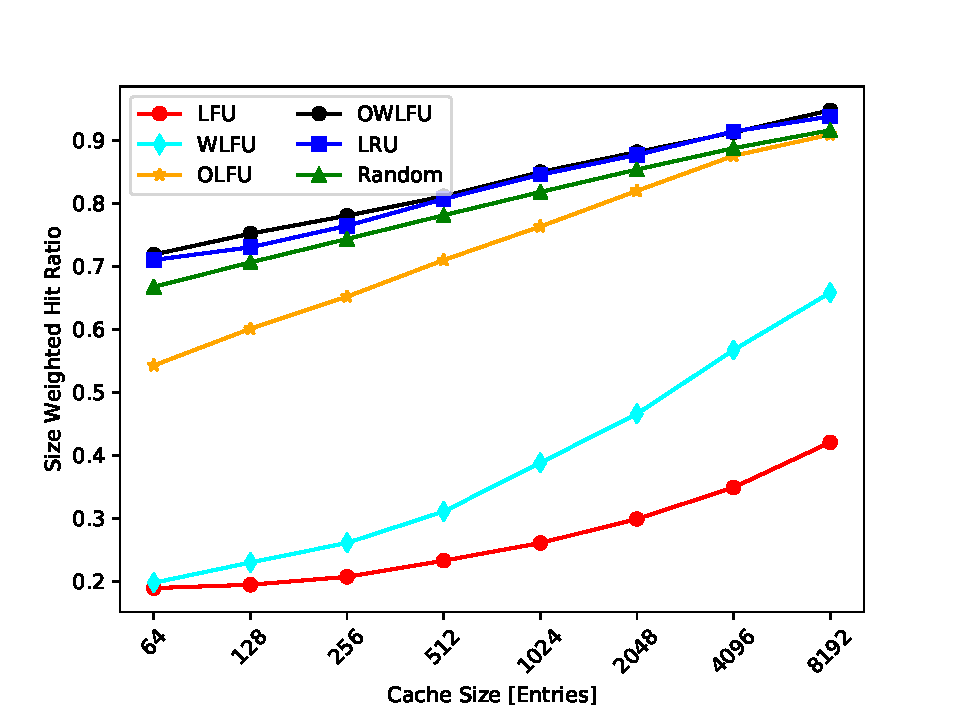
\includegraphics[width=0.33\textwidth]{weighted_hit_ratio_sf1.pdf}
\label{fig:weighted_hit_ratio_sf1}
}
\subfloat[Size Weighted Hit Ratio. Slowdown factor = 10]{
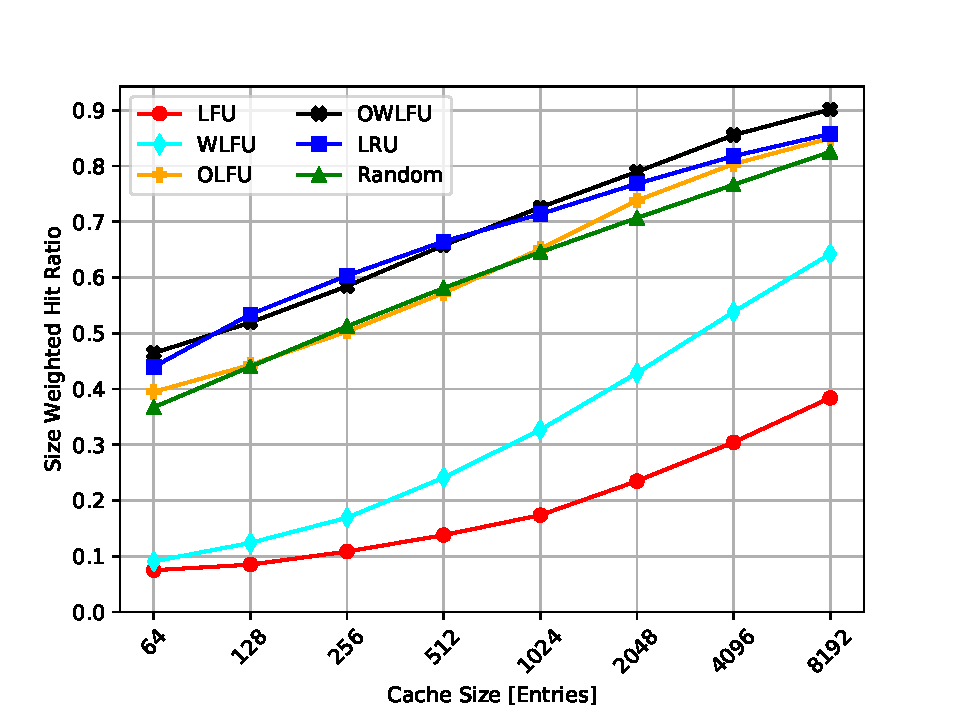
\includegraphics[width=0.33\textwidth]{weighted_hit_ratio_sf10.pdf}
\label{fig:weighted_hit_ratio_sf10}
}
\subfloat[Size Weighted Hit Ratio. Slowdown factor = 100]{
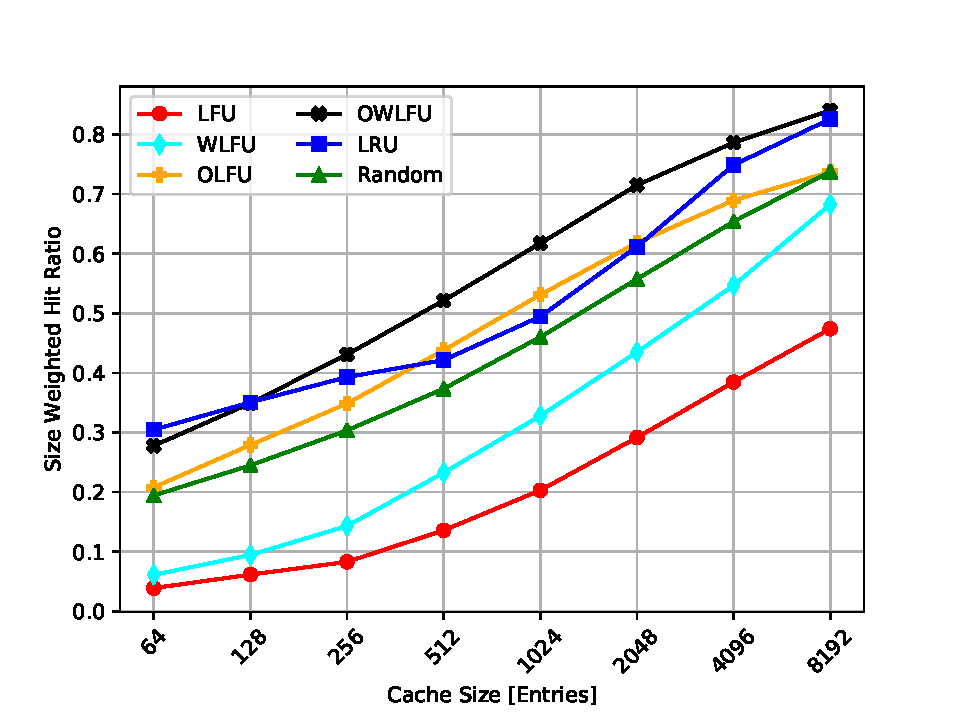
\includegraphics[width=0.33\textwidth]{weighted_hit_ratio_sf100.pdf}
\label{fig:weighted_hit_ratio_sf100}
}
\caption{Cache performance evaluation}
\label{fig:hit_ratio}
\end{figure*}